\section{Phân tích What-Why}

\subsection{Bảng phân tích biến số (Variable types)}

Dưới đây là bảng chi tiết các biến trong bộ dữ liệu e-commerce cùng với vai trò và kiểu dữ liệu:

\begin{table}[H]
\centering
\renewcommand{\arraystretch}{1.3}
\begin{tabularx}{\textwidth}{|l|L{3.5cm}|X|}
    \hline
    \textbf{Biến} & \textbf{Kiểu dữ liệu} & \textbf{Mô tả} \\
    \hline
    \texttt{order\_id} & Categorical (Nominal) & Mã đơn hàng --- mã duy nhất cho mỗi giao dịch. \\
    \hline
    \texttt{customer\_id} & Categorical (Nominal) & Mã khách hàng --- mã duy nhất cho mỗi khách hàng. \\
    \hline
    \texttt{product\_id} & Categorical (Nominal) & Mã sản phẩm --- mã duy nhất cho mỗi sản phẩm. \\
    \hline
    \texttt{category} & Categorical (Nominal) & Danh mục sản phẩm (Electronics, Fashion, Home, Beauty, Sports, Toys, Grocery). \\
    \hline
    \texttt{price} & Quantitative (Ratio) & Đơn giá sản phẩm. \\
    \hline
    \texttt{discount} & Quantitative (Ratio) & Phần trăm giảm giá được áp dụng (\%). \\
    \hline
    \texttt{quantity} & Quantitative (Ratio) & Số lượng sản phẩm trong mỗi đơn hàng. \\
    \hline
    \texttt{order\_date} & Ordered (Temporal) & Ngày đặt hàng. \\
    \hline
    \texttt{delivery\_time\_days} & Quantitative (Ratio) & Số ngày giao hàng. \\
    \hline
    \texttt{region} & Categorical (Nominal) & Khu vực địa lý của khách hàng. \\
    \hline
    \texttt{returned} & Categorical (Binary) & Sản phẩm có bị trả lại (Yes/No). \\
    \hline
    \texttt{total\_amount} & Quantitative (Ratio) & Tổng tiền thanh toán sau khi giảm giá. \\
    \hline
    \texttt{profit\_margin} & Quantitative (Ratio) & Biên lợi nhuận của đơn hàng. \\
    \hline
    \texttt{customer\_age} & Quantitative (Ratio) & Tuổi của khách hàng (18--70). \\
    \hline
    \texttt{customer\_gender} & Categorical (Nominal) & Giới tính khách hàng. \\
    \hline
\end{tabularx}
\caption{Bảng phân loại các biến số và vai trò phân tích}
\end{table}

\subsection{Phân tích Why (Nhiệm vụ / Câu hỏi phân tích)}

Dưới đây là các câu hỏi phân tích dự kiến mà Dashboard sẽ trả lời:

\subsubsection{Nhóm 1: Xu hướng Doanh thu theo Thời gian}

\begin{enumerate}
    \item \textbf{Doanh thu thay đổi như thế nào theo từng tháng/quý?} Có xu hướng tăng trưởng hay suy giảm không?
    \item \textbf{Tháng nào trong năm có doanh thu cao nhất?} Có yếu tố mùa vụ (seasonality) rõ ràng không?
    \item \textbf{Ngày nào trong tuần có nhiều đơn hàng nhất?} Xu hướng mua sắm theo thời gian ra sao?
\end{enumerate}

% --- tv1_duc.tex ---
% Phân tích Nhóm 1: Xu hướng Doanh thu theo Thời gian
\newpage
\vspace{0.6cm}
\noindent\textbf{3. Kết quả phân tích \& Trực quan hóa:}

% (a) Biến động theo tháng/quý
\begin{enumerate}[label=(\alph*)]
    \item \textbf{Biến động theo tháng/quý:}
\end{enumerate}

\begin{figure}[H]
    \centering
    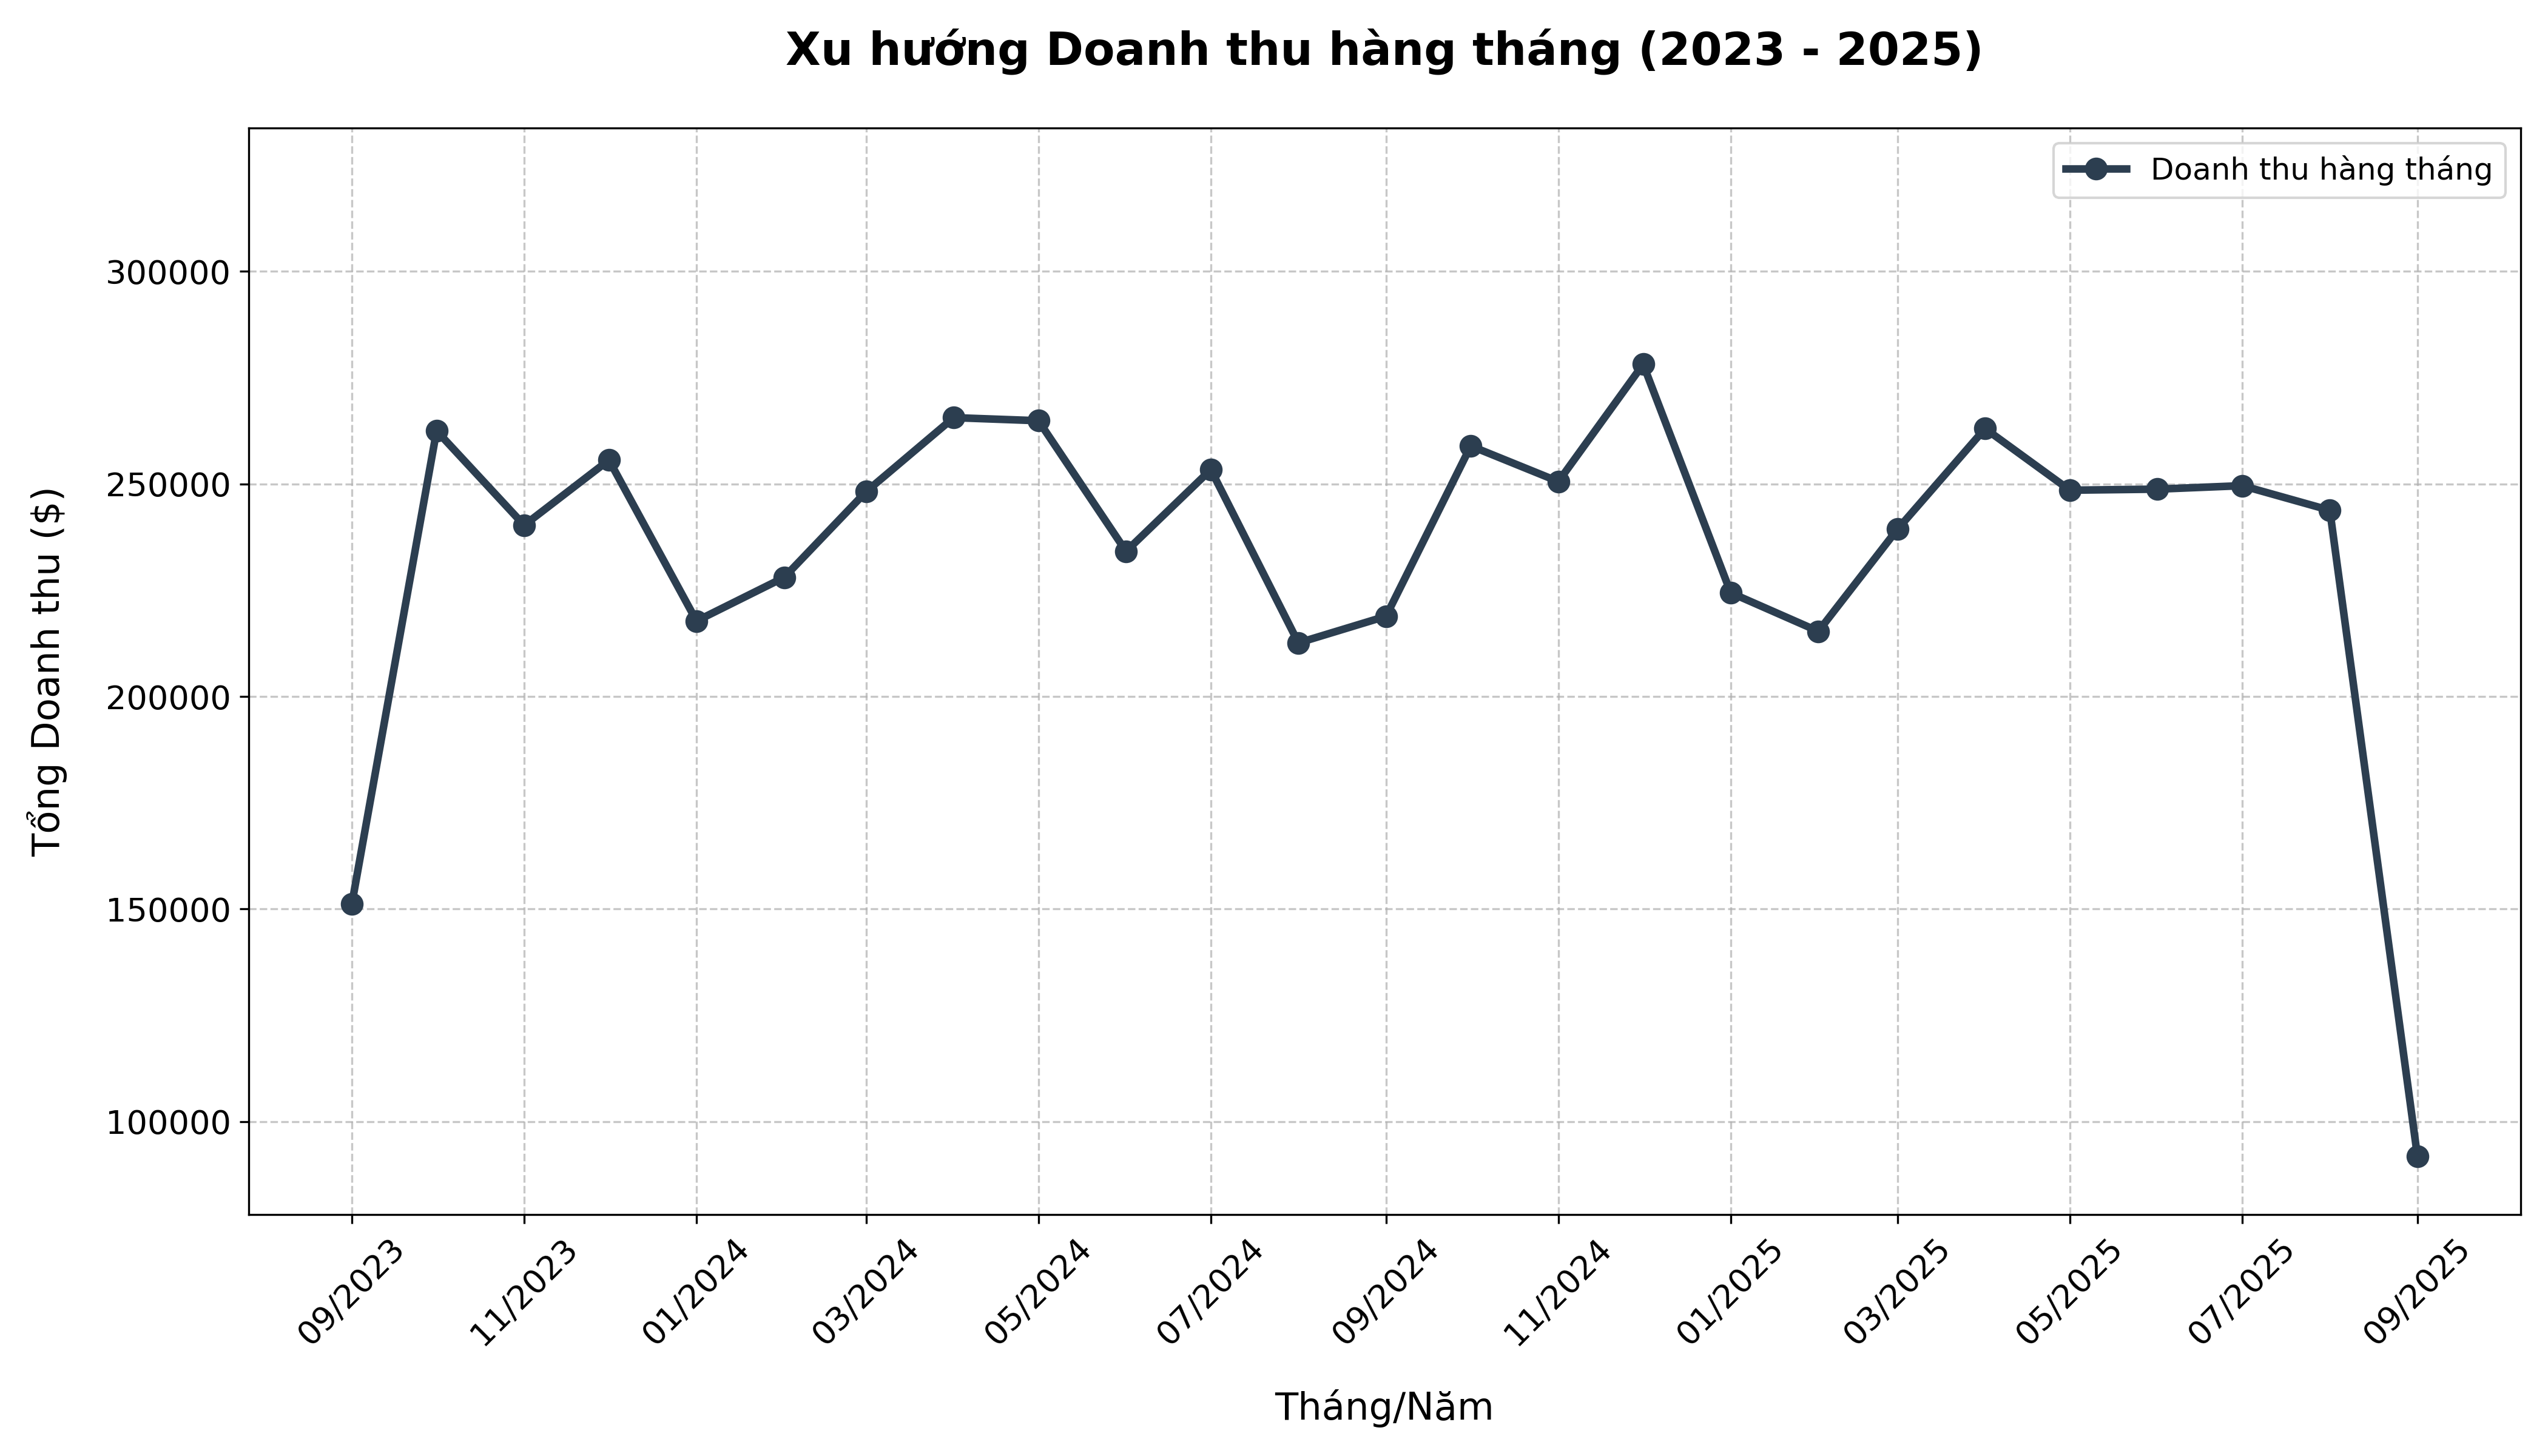
\includegraphics[width=1\textwidth]{images/revenue_trend.png}
    \caption{Biểu đồ xu hướng doanh thu hàng tháng từ 2023 - 2025}
    \label{fig:revenue_trend}
\end{figure}

\begin{itemize}
    \item \textbf{Biến động theo Tháng (Monthly Trend):}
    \begin{itemize}[label=--]
        \item \textit{Xu hướng tổng thể:} Doanh thu duy trì ở mức ổn định nhưng có xu hướng biến động mạnh theo từng tháng. Đặc biệt, điểm thấp nhất toàn kỳ rơi vào \textbf{tháng 9/2025}, đánh dấu sự sụt giảm đáng kể so với các giai đoạn trước đó.
        \item \textit{Các đợt biến động:} Ghi nhận sự tăng trưởng trở lại ngay sau các giai đoạn thấp điểm, cho thấy khả năng phục hồi nhanh của thị trường.
    \end{itemize}
\end{itemize}

\begin{figure}[H]
    \centering
    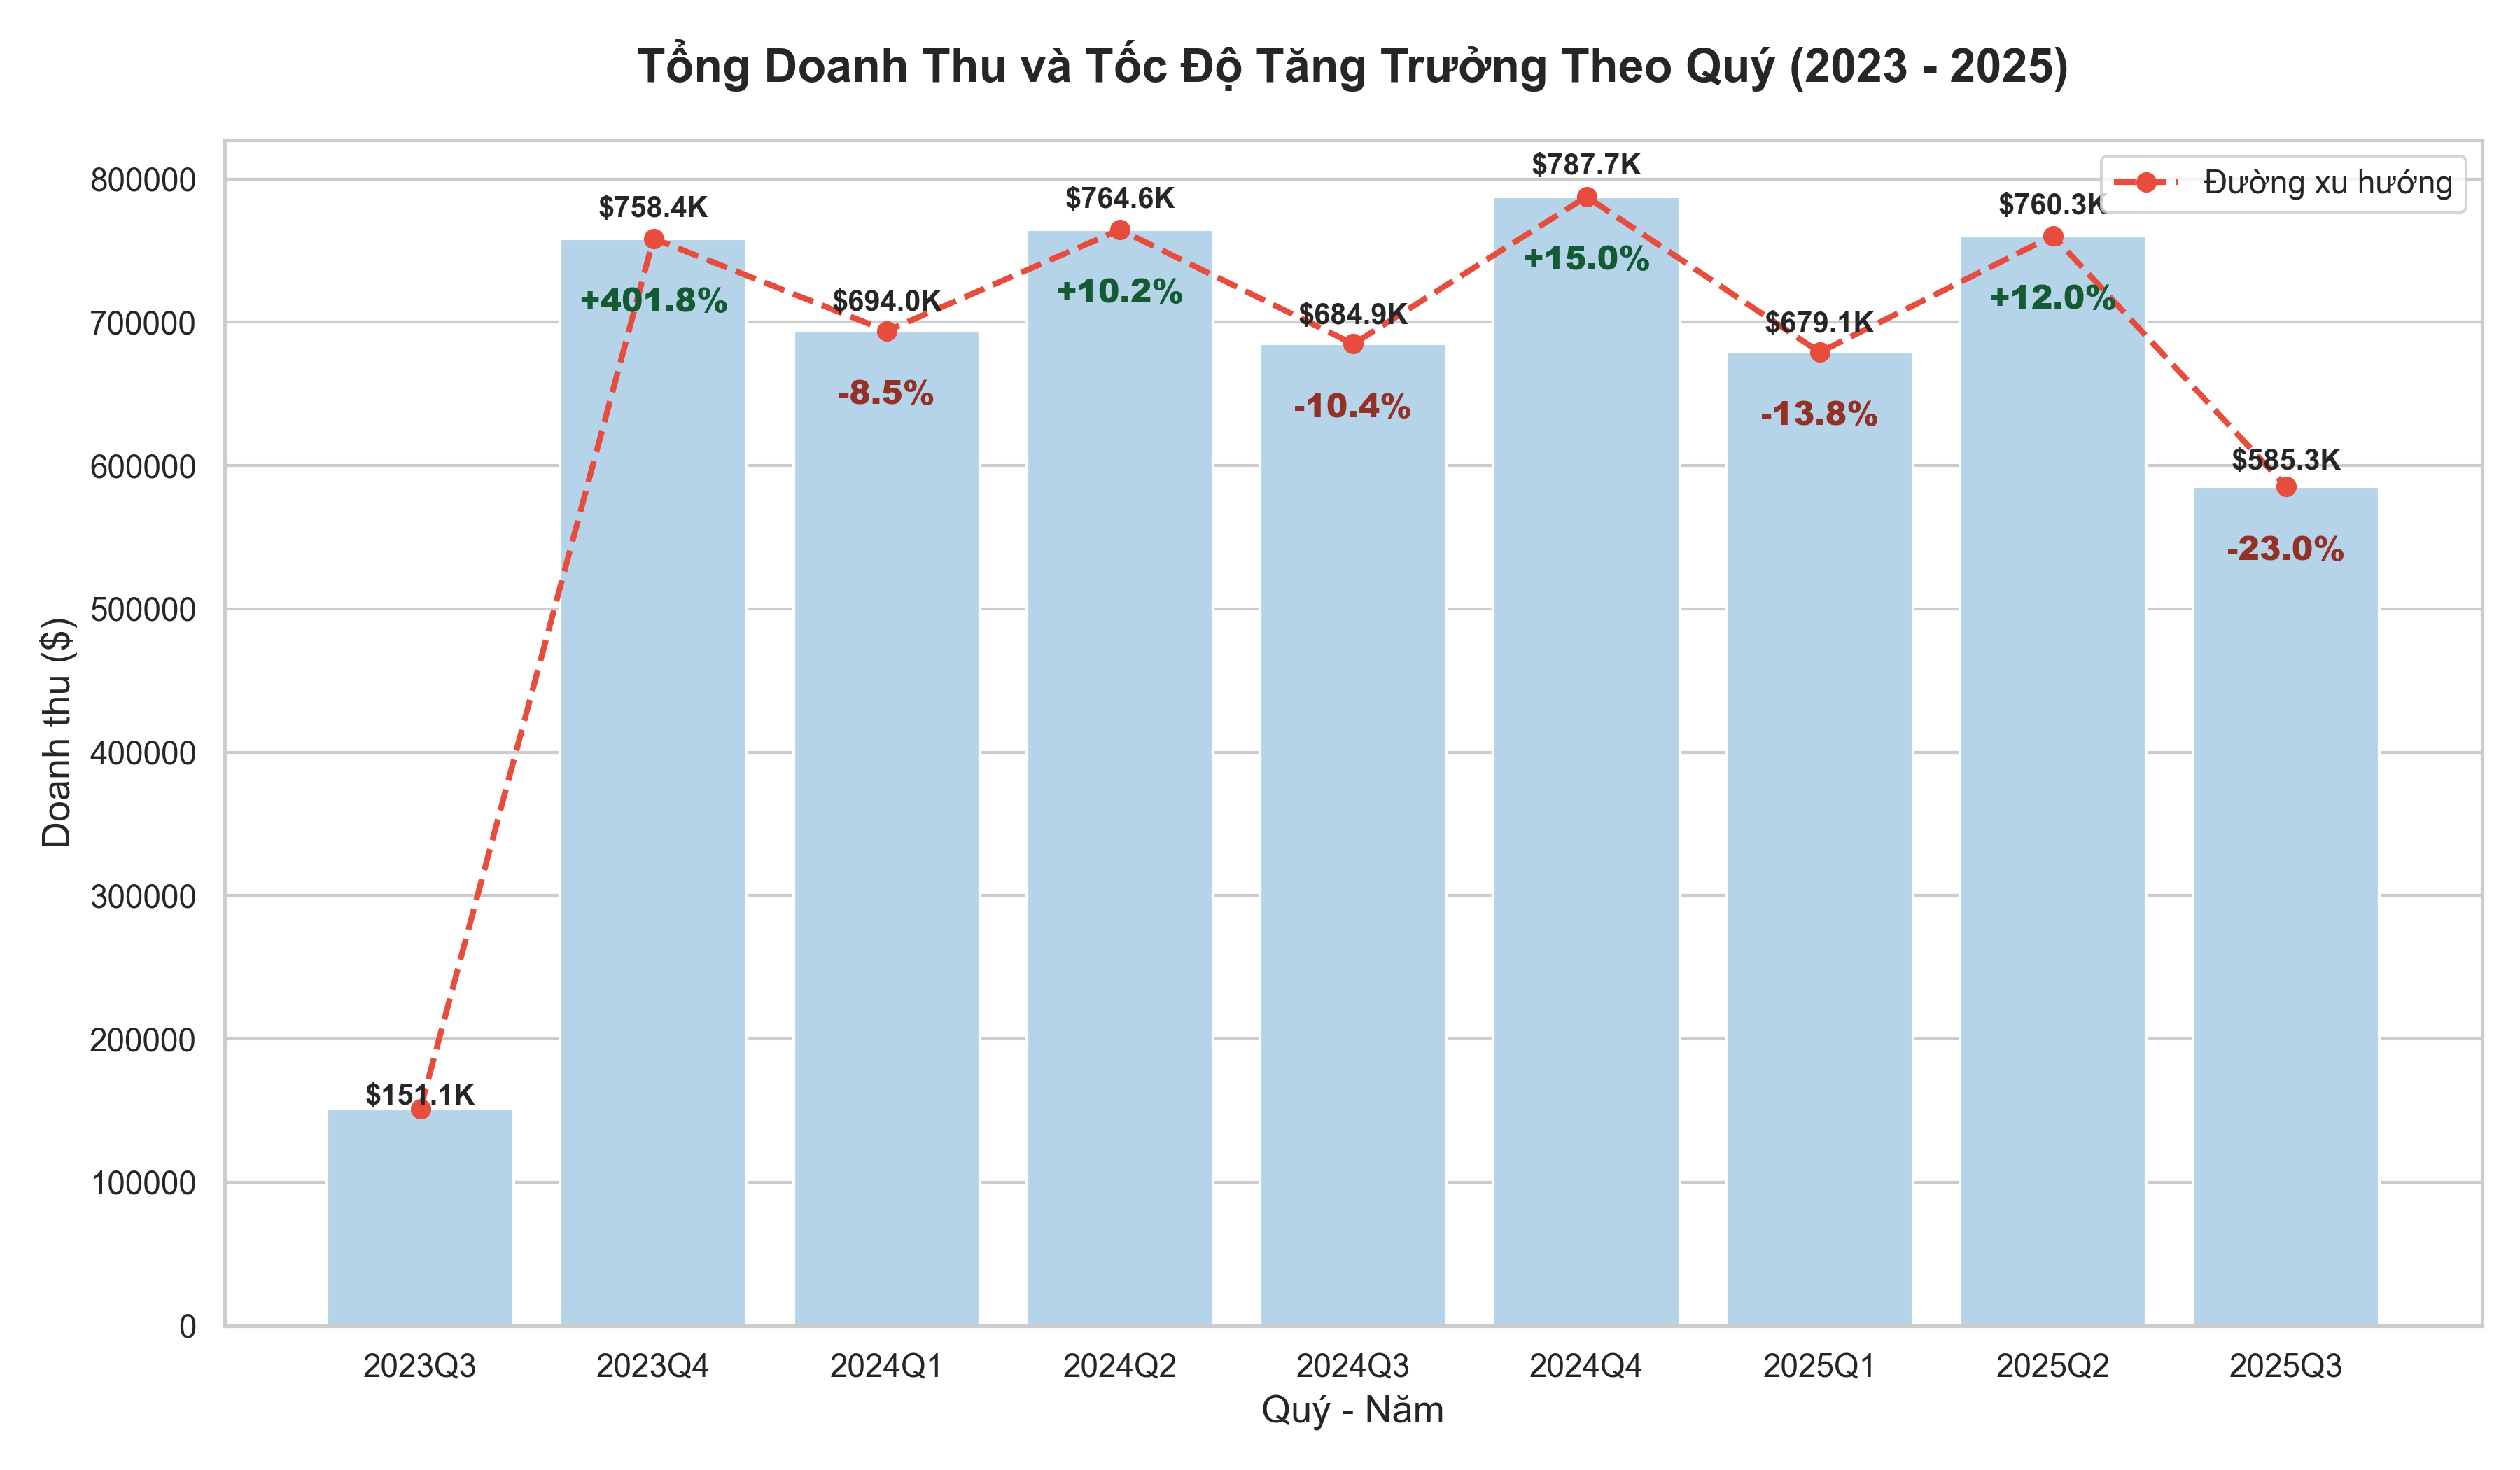
\includegraphics[width=1\textwidth]{images/quarterly_revenue.png}
    \caption{Biểu đồ tổng doanh thu và tốc độ tăng trưởng theo quý}
    \label{fig:quarterly_revenue}
\end{figure}

\begin{itemize}
    \item \textbf{Biến động và Tăng trưởng theo Quý (Quarterly Growth):}
    \begin{itemize}[label=--]
        \item \textit{Tăng trưởng 2024:} Năm 2024 ghi nhận sự bứt phá mạnh mẽ vào \textbf{Quý 2 (+10.2\%)} và đặc biệt là \textbf{Quý 4 (+15.0\%)} - đạt mức doanh thu kỷ lục \$787.7K.
        \item \textit{Các đợt điều chỉnh:} Ngược lại, doanh thu suy giảm vào Quý 1 (-8.5\%) và Quý 3 (-10.4\%), cho thấy tính biến động của thị trường theo từng giai đoạn ngắn hạn trước khi bùng nổ vào cuối năm.
    \end{itemize}
\end{itemize}

% (b) Tháng cao điểm & Mùa vụ
\begin{enumerate}[label=(\alph*), resume]
    \item \textbf{Tháng cao điểm \& Mùa vụ:}
\end{enumerate}

\begin{figure}[H]
    \centering
    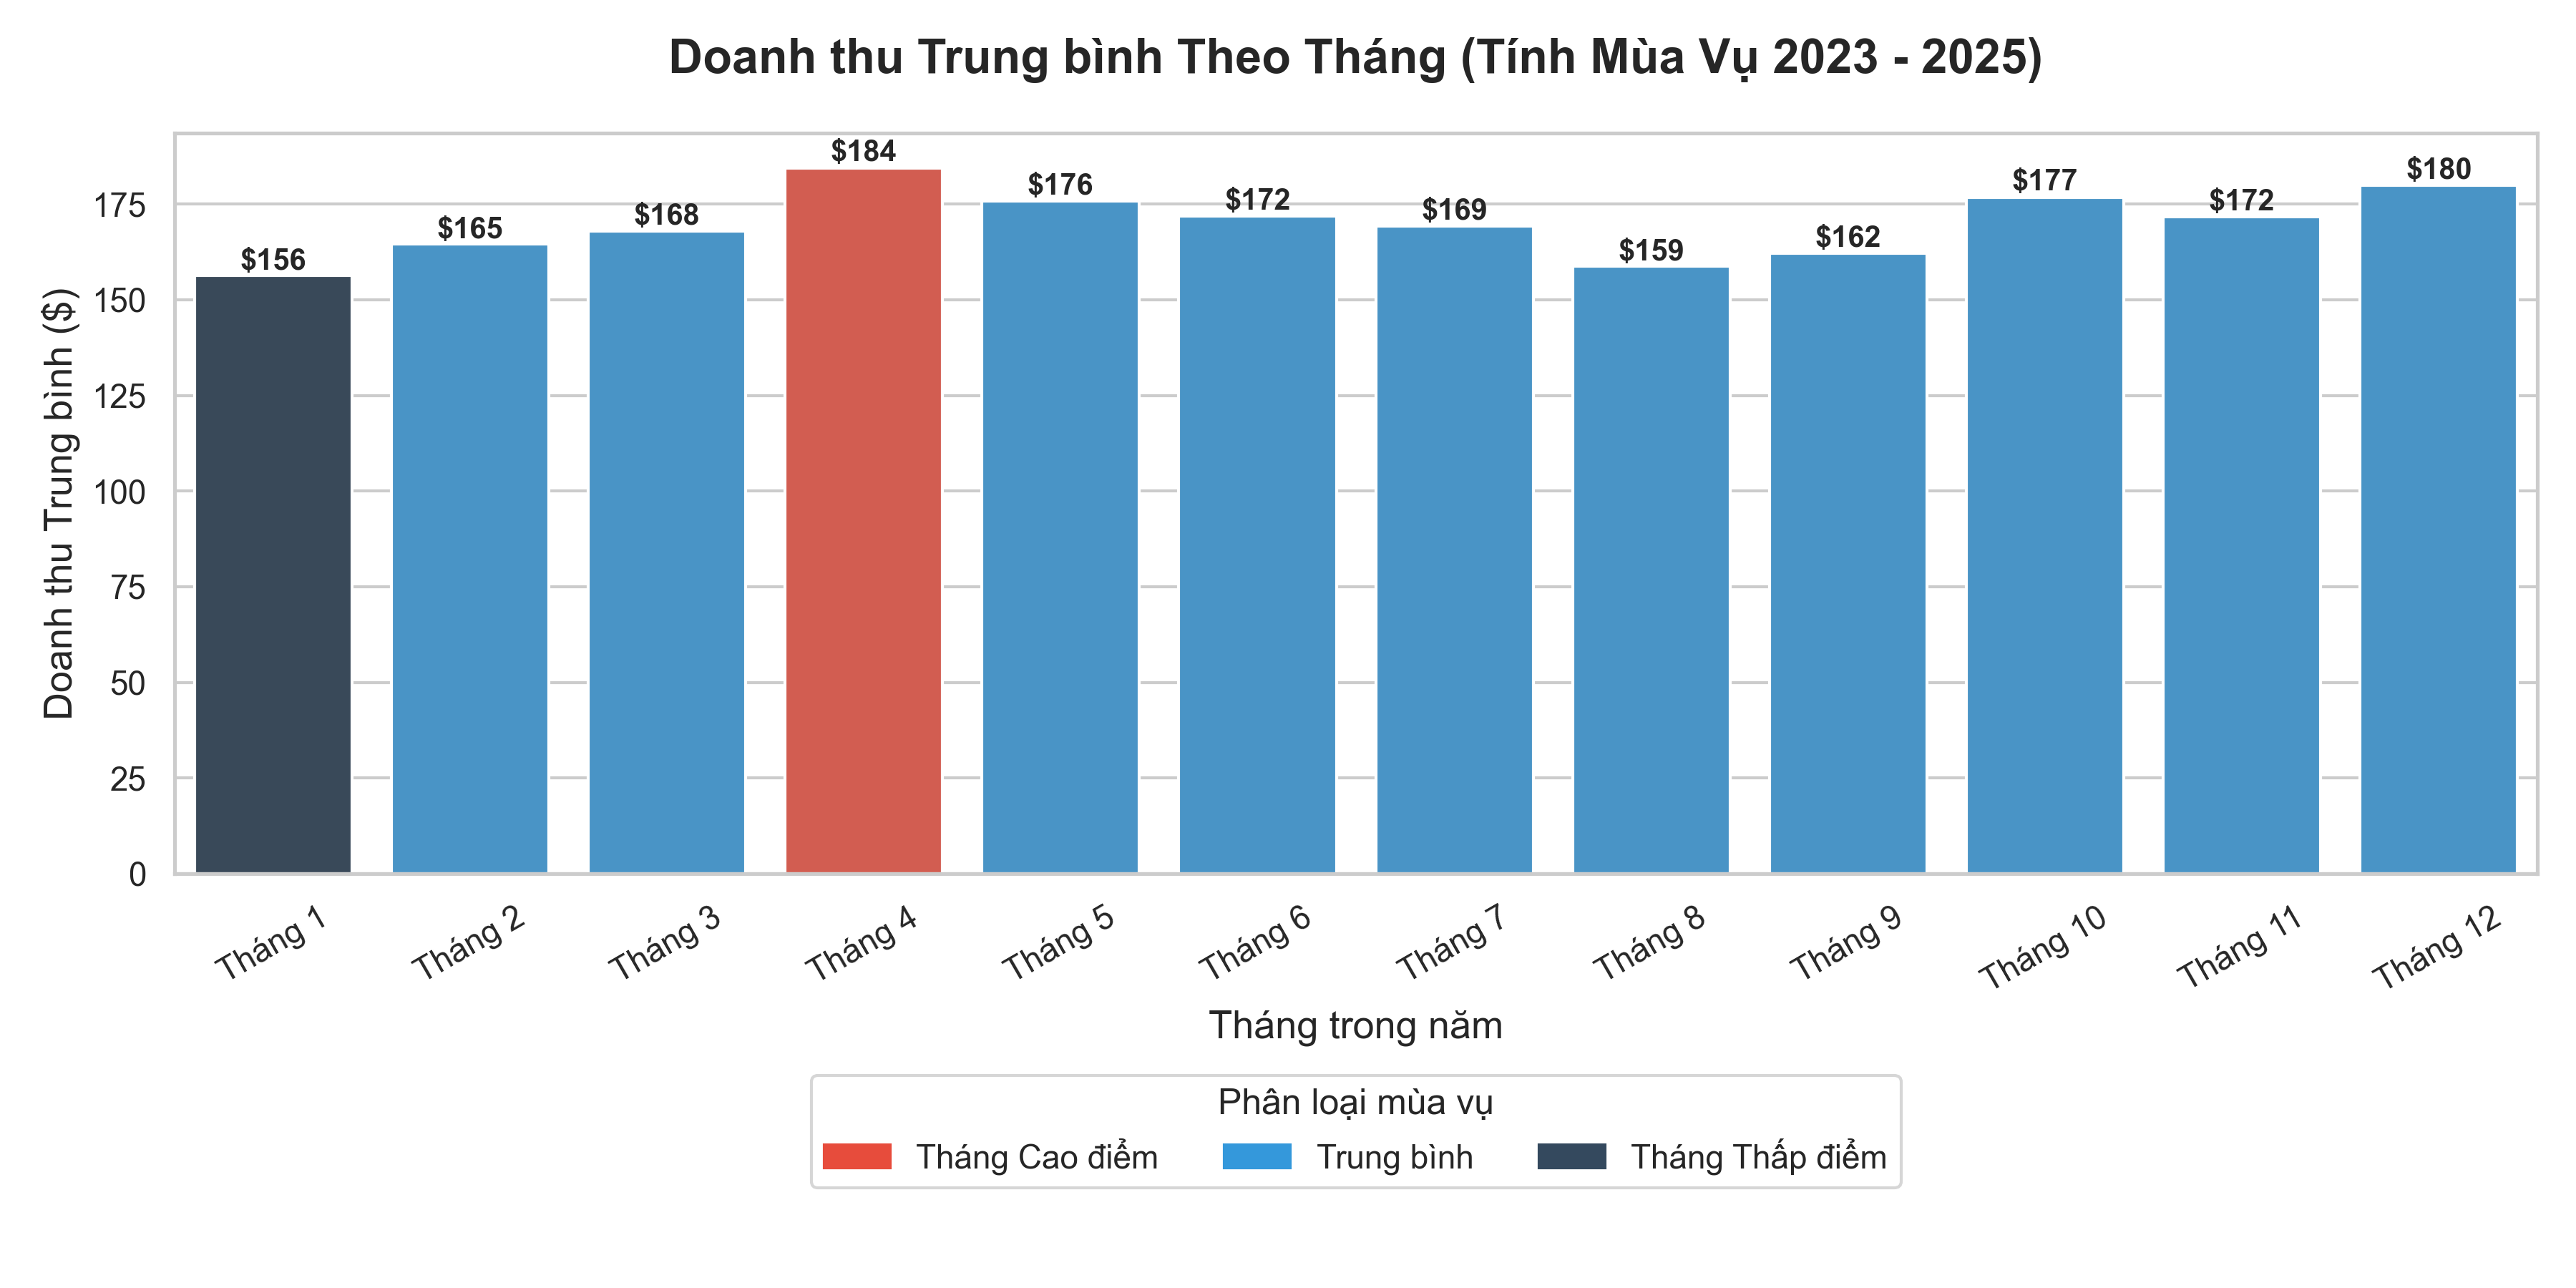
\includegraphics[width=1\textwidth]{images/seasonal_revenue.png}
    \caption{Doanh thu trung bình theo tháng}
    \label{fig:seasonal_revenue}
\end{figure}

\begin{itemize}
    \item \textit{Cao điểm:} Dữ liệu trung bình nhiều năm xác nhận \textbf{Tháng 12 và Tháng 10} là hai tháng mang lại doanh thu cao nhất (trên \$160,000/tháng). Tháng 4 cũng là một điểm sáng mùa vụ quan trọng.
    \item \textit{Thấp điểm:} \textbf{Tháng 1} là tháng có doanh thu trung bình thấp nhất, khớp với biểu đồ mùa vụ (màu xám đậm), phản ánh sự bão hòa chi tiêu sau Tết/Lễ hội.
\end{itemize}

% (c) Xu hướng theo tuần
\begin{enumerate}[label=(\alph*), resume]
    \item \textbf{Xu hướng theo tuần:}
\end{enumerate}

\begin{figure}[H]
    \centering
    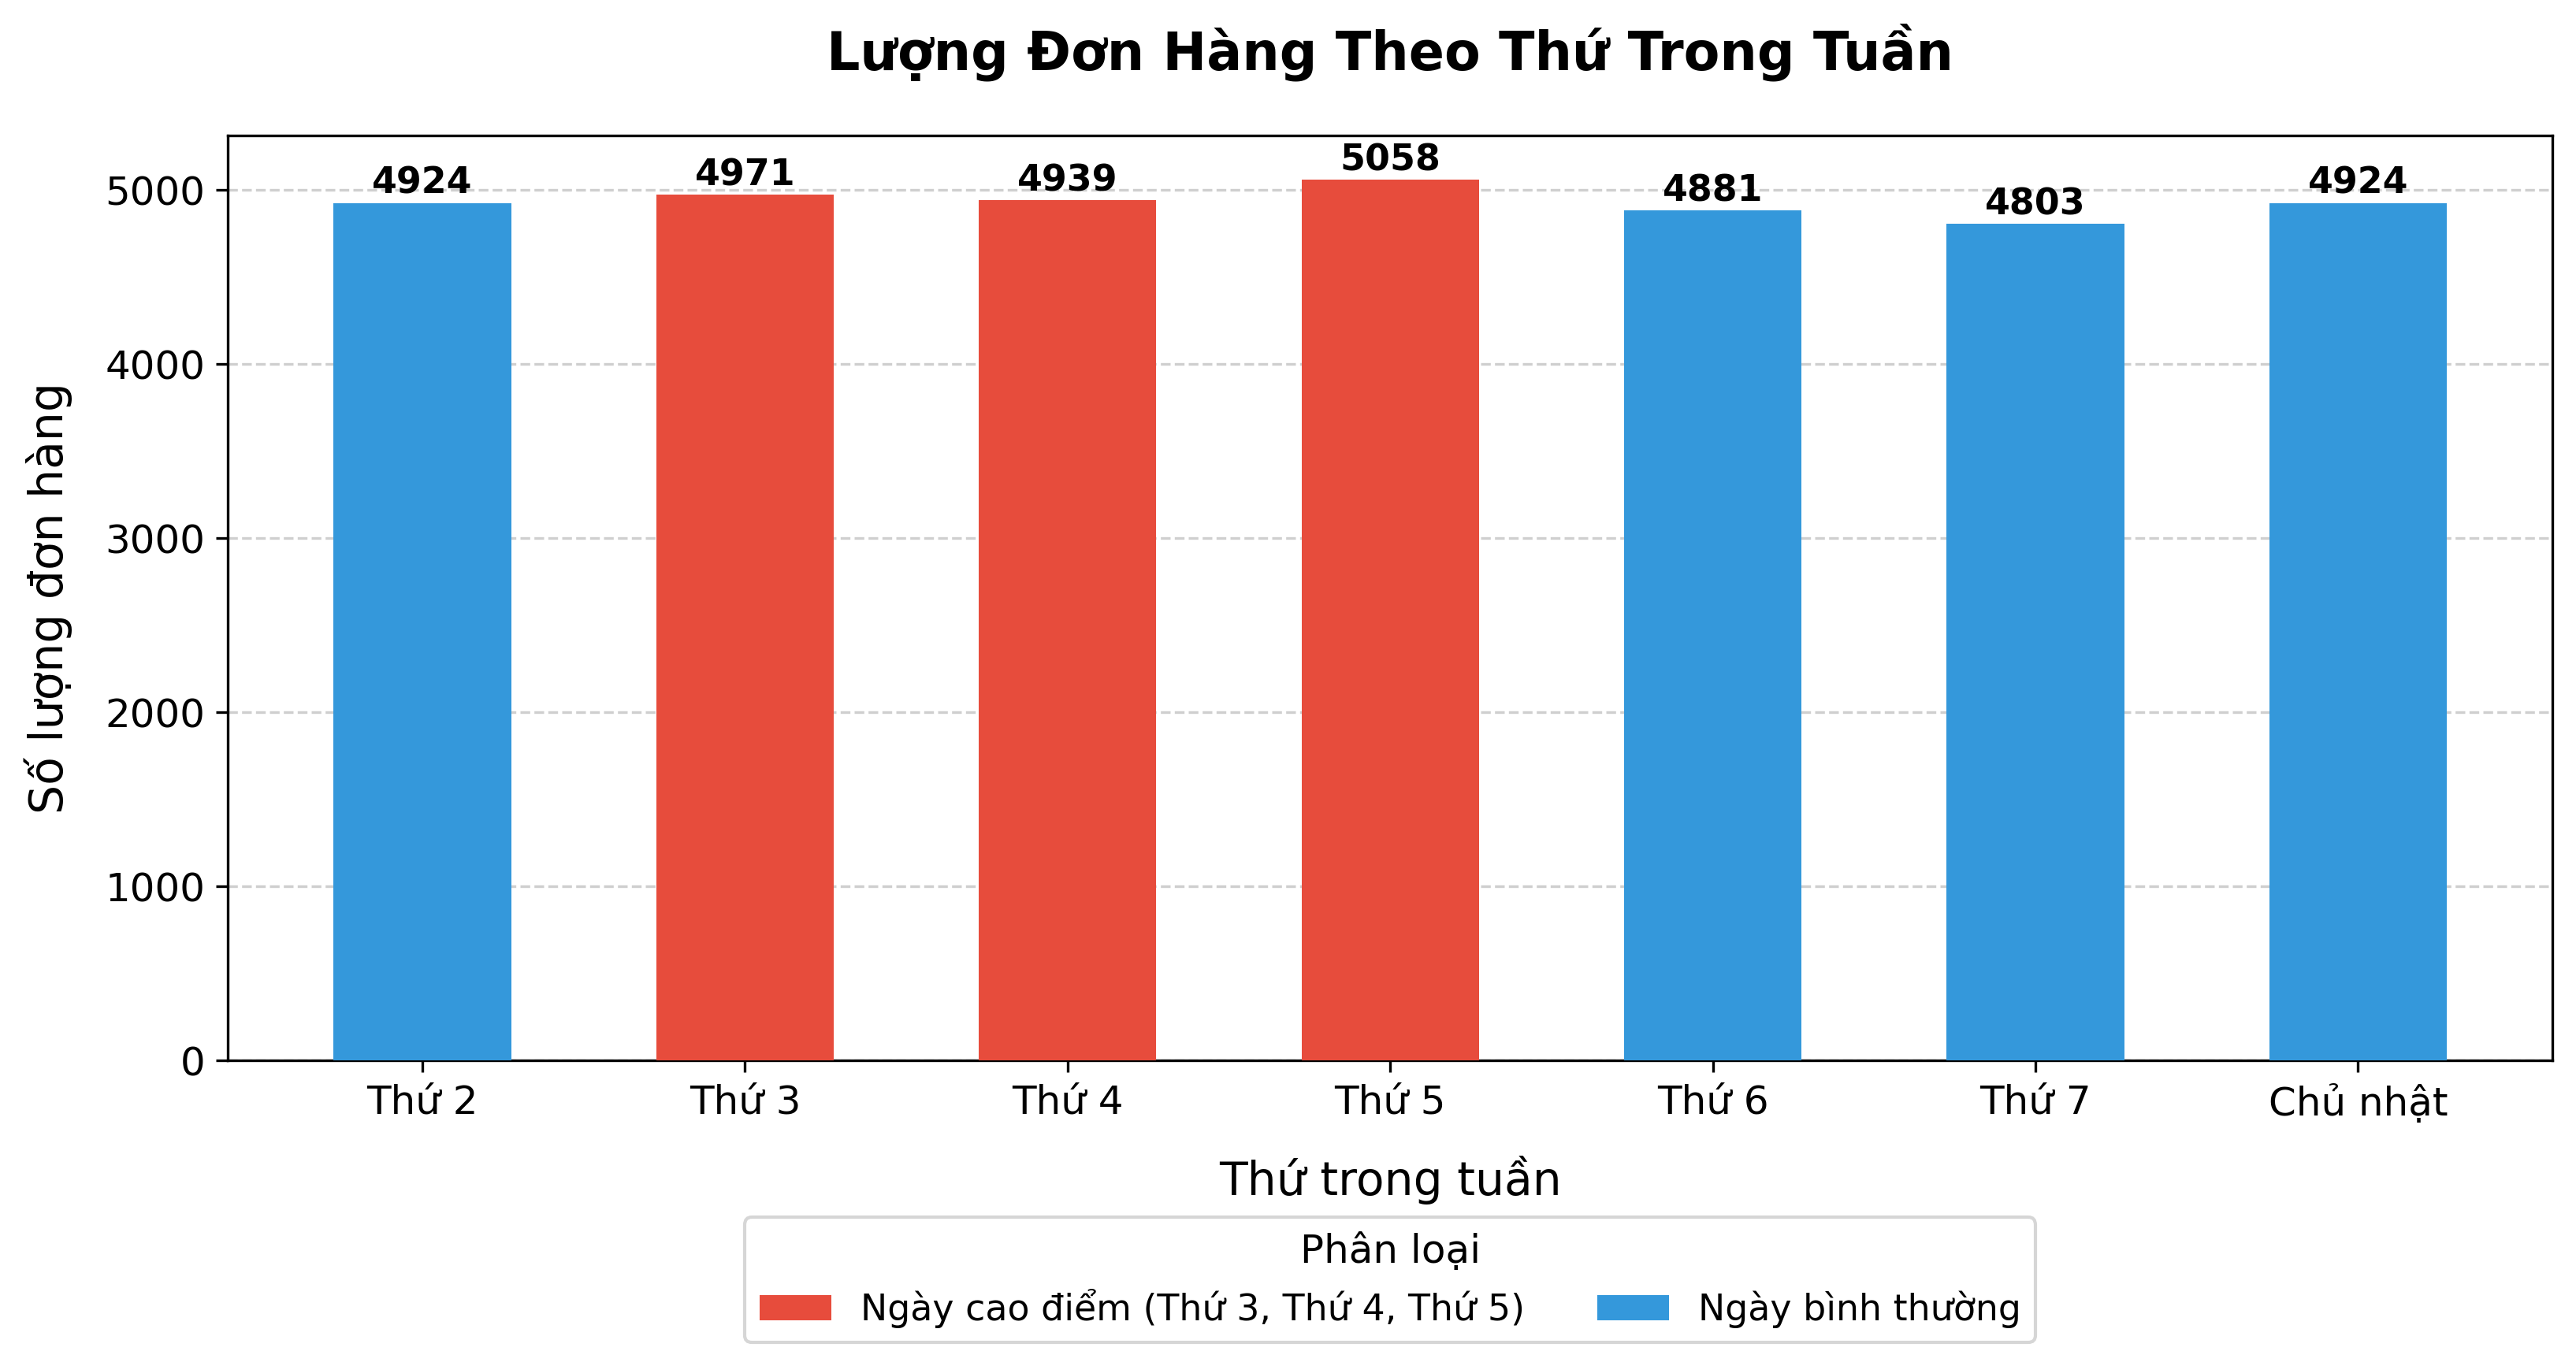
\includegraphics[width=0.88\textwidth]{images/dow_trend.png}
    \caption{Lượng đơn hàng phân bổ theo các thứ trong tuần}
    \label{fig:dow_trend}
\end{figure}

\begin{itemize}
    \item Nhìn vào biểu đồ cột, có thể thấy rõ \textbf{Thứ Ba, Thứ Tư và Thứ Năm} là các ngày cao điểm nhất trong tuần (trong đó Thứ Năm vượt mốc 5,000 đơn hàng). Lượng giao dịch tập trung cực lớn vào giai đoạn giữa tuần, trong khi các ngày cuối tuần (Thứ Bảy, Chủ Nhật) lại có lượng giao dịch thấp hơn. Điều này cho thấy thói quen mua sắm trực tuyến gắn liền với thời gian làm việc hành chính của khách hàng.
\end{itemize}

\vspace{0.3cm}
\noindent\textbf{4. Đưa ra quyết định trong tương lai:}
\begin{itemize}
    \item \textbf{Quản lý kho vận (Inventory):} Tăng cường dự trữ hàng hóa từ tháng 9 để chuẩn bị cho cao điểm quý IV. Đặc biệt chú trọng các mặt hàng chủ chốt vào tháng 4.
    \item \textbf{Chiến lược Marketing:} Đẩy mạnh các chương trình khuyến mãi vào giai đoạn đầu năm (tháng 1 và tháng 2) để kích cầu trong thời kỳ thấp điểm.
    \item \textbf{Tối ưu hóa nhân sự:} Phân bổ thêm nhân lực xử lý đơn hàng vào các ngày giữa tuần để đảm bảo thời gian giao hàng nhanh nhất.
\end{itemize}

\subsubsection{Nhóm 2: Phân tích Sản phẩm \& Danh mục}

\begin{enumerate}
    \setcounter{enumi}{3}
    \item \textbf{Danh mục nào có doanh thu cao nhất?} So sánh doanh thu giữa 7 danh mục (Electronics, Fashion, Home, Beauty, Sports, Toys, Grocery).
    \item \textbf{Tỷ lệ hoàn trả theo từng danh mục là bao nhiêu?} Danh mục nào có tỷ lệ hoàn trả cao nhất?
    \item \textbf{Mức giảm giá ảnh hưởng thế nào đến doanh thu và biên lợi nhuận?}
\end{enumerate}

% --- tv2_quangvinh.tex ---
% Phân tích Nhóm 2: Phân tích Sản phẩm & Danh mục

\noindent\textbf{3. Kết quả phân tích \& Trực quan hóa:}

\begin{figure}[H]
    \centering
    
\includegraphics[width=0.8\textwidth]{images/category_finance/cat_revenue.png}
    \caption{Tổng doanh thu theo từng danh mục sản phẩm}
    \label{fig:cat_revenue}
\end{figure}

\textbf{a. Phân tích Doanh thu theo Danh mục}
\\
Biểu đồ \ref{fig:cat_revenue} cho thấy sự phân hóa cực kỳ rõ rệt về doanh thu giữa các nhóm ngành hàng. Danh mục \textbf{Electronics (Điện tử)} áp đảo hoàn toàn với tổng doanh thu đạt mức \$3.31 triệu, cao gấp 3 lần so với nhóm xếp thứ hai là \textbf{Home (Nhà cửa)} (\$1.07 triệu). Các nhóm hàng tiêu dùng thiết yếu như Grocery (Tạp hóa) lại có doanh thu thấp nhất (\$82 nghìn). Điều này chỉ ra rằng các sản phẩm điện tử, dù có số lượng giao dịch thể không quá cao, nhưng nhờ đơn giá lớn đã mang lại nguồn thu khổng lồ cho nền tảng.

\begin{figure}[H]
    \centering
    
\includegraphics[width=0.8\textwidth]{images/category_finance/cat_return_rate.png}
    \caption{Tỷ lệ hoàn trả (Return Rate) theo danh mục}
    \label{fig:cat_return}
\end{figure}

\textbf{b. Phân tích Rủi ro Hoàn trả (Return Rate)}
\\
Biểu đồ \ref{fig:cat_return} thể hiện phần trăm các đơn hàng bị trả lại trên tổng số đơn. Có một điều đáng lưu ý là \textbf{Fashion (Thời trang)} dẫn đầu bảng với tỷ lệ hoàn trả cao nhất lên tới 8.28\%, theo ngay sau là \textbf{Electronics} (7.29\%). Đối với ngành thời trang, tỷ lệ trả hàng cao thường xuất phát từ vấn đề sai lệch kích cỡ hoặc không ưng ý về kiểu dáng. Đối với đồ điện tử, đây có thể là rủi ro liên quan đến lỗi kỹ thuật. Trong khi đó, nhóm \textbf{Grocery} có tỷ lệ trả hàng thấp nhất (chỉ 1.3\%), cho thấy vòng đời sử dụng nhanh và ít sai số.

\begin{figure}[H]
    \centering
    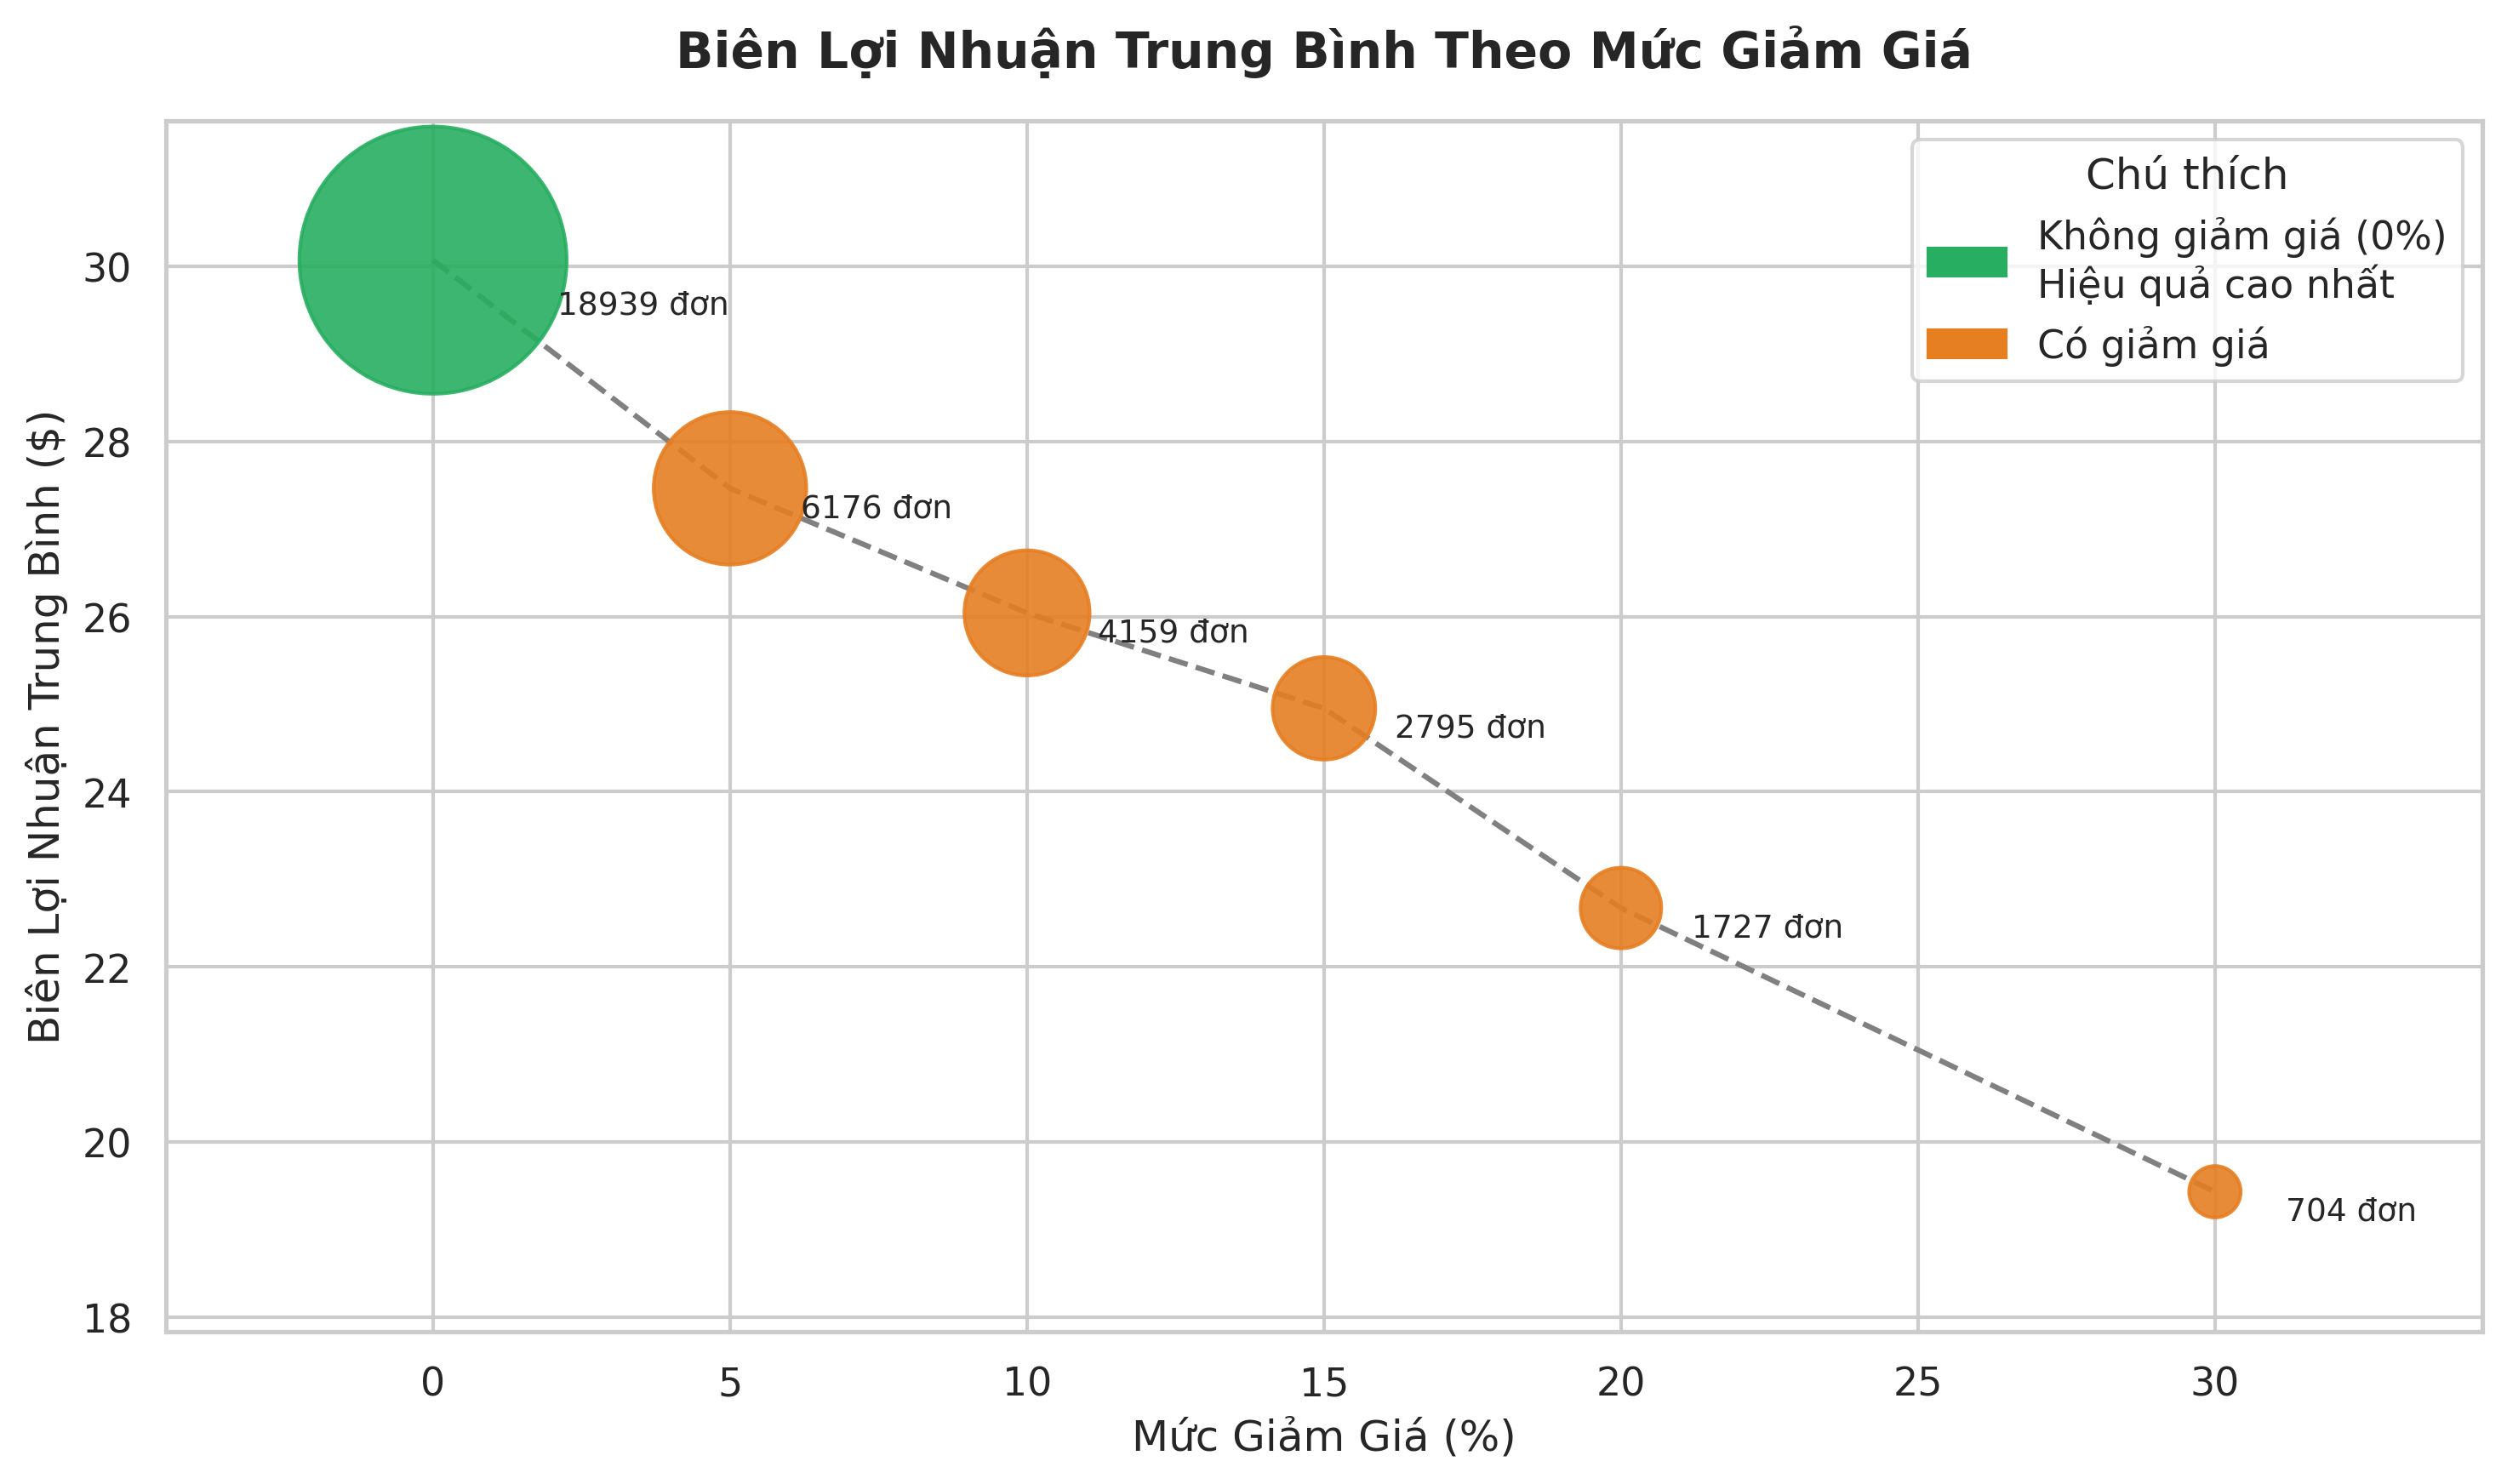
\includegraphics[width=0.8\textwidth]{images/category_finance/discount_profit.png}
    \caption{Mối tương quan giữa phần trăm giảm giá và biên lợi nhuận trung bình}
    \label{fig:discount_profit}
\end{figure}

\textbf{c. Tương quan giữa Mức Giảm Giá và Biên Lợi Nhuận}
\\
Thông qua biểu đồ phân tán \ref{fig:discount_profit} (kích thước điểm ảnh biểu diễn số lượng đơn hàng), ta dễ dàng nhận thấy một quy luật tuyến tính nghịch biến: \textbf{Mức giảm giá càng cao, biên lợi nhuận trung bình cho mỗi đơn hàng càng giảm}.
Đáng chú ý, đa số các đơn hàng (gần 19,000 đơn) không áp dụng mã giảm giá (0\%) và đem lại biên lợi nhuận cao nhất (khoảng \$30.07). Trong khi đó, các mức giảm giá sâu như 30\% khiến biên lợi nhuận sụt giảm xuống chỉ còn \$19.42 và số lượng giao dịch tại mức này cũng rất ít (hơn 700 đơn). Do đó, doanh nghiệp cần cân nhắc kỹ việc lạm dụng khuyến mãi sâu vì nó gây tổn thất đáng kể đến lợi nhuận ròng mà không tạo ra đột biến ấn tượng về số lượng đơn hàng.

\vspace{0.3cm}
\noindent\textbf{4. Đưa ra quyết định trong tương lai:}
\begin{itemize}
    \item \textbf{Tối ưu danh mục chủ lực:} Tập trung nguồn lực marketing và đa dạng hóa mẫu mã cho nhóm \textbf{Electronics} vì đây là "mỏ neo" doanh thu chính. Tuy nhiên, cần thắt chặt kiểm tra kỹ thuật trước khi giao để giảm tỷ lệ hoàn trả (7.29\%).
    \item \textbf{Cải thiện chất lượng ngành Fashion:} Triển khai thêm các công cụ hỗ trợ chọn size hoặc mô tả chi tiết hơn để giảm thiểu tỷ lệ hoàn trả cao nhất hệ thống (8.28\%).
    \item \textbf{Chiến lược chiết khấu:} Ưu tiên các mức giảm giá từ 0--10\% để duy trì biên lợi nhuận ổn định. Tránh các chương trình giảm giá sâu (trên 20\%) trừ khi mục tiêu là xả kho vì hiệu quả mang lại về lợi nhuận là không cao.
\end{itemize}



\subsubsection{Nhóm 3: Phân tích Khách hàng}

\begin{enumerate}
    \setcounter{enumi}{6}
    \item \textbf{Phân bổ khách hàng theo độ tuổi và giới tính như thế nào?} Nhóm nào chi tiêu nhiều nhất?
    \item \textbf{Phương thức thanh toán nào được ưa chuộng nhất?} Có sự khác biệt theo nhóm tuổi/giới tính không?
    \item \textbf{Top khách hàng có giá trị cao nhất (theo tổng chi tiêu) là ai?}
\end{enumerate}

% --- tv3_quocviet.tex ---
% Phân tích Nhóm 3: Phân tích Khách hàng

\noindent\textbf{3. Kết quả phân tích \& Trực quan hóa:}

\begin{figure}[H]
    \centering
    
\includegraphics[width=0.9\textwidth]{images/customer_analysis/cust_spend_age_gender.png}
    \caption{Tổng chi tiêu theo nhóm tuổi và giới tính}
    \label{fig:cust_spend_age_gender}
\end{figure}

\textbf{a. Phân bổ khách hàng theo độ tuổi và giới tính --- Nhóm nào chi tiêu nhiều nhất?}
\\
Biểu đồ \ref{fig:cust_spend_age_gender} sử dụng Grouped Bar Chart với trục X là nhóm tuổi (18--24, 25--34, 35--44, 45--54, 55--69), chiều cao cột biểu thị tổng chi tiêu khả dụng (nghìn USD, đã loại trừ đơn hàng hoàn trả) và màu sắc phân biệt giới tính. Kết quả cho thấy \textbf{nhóm 55--69 tuổi chi tiêu cao nhất} với mức \$748K (Female) và \$718K (Male), phản ánh sức mua vượt trội của nhóm khách hàng đã tích lũy thu nhập ổn định. Ngược lại, nhóm \textbf{18--24 tuổi} có chi tiêu thấp nhất toàn sàn (Female: \$376K, Male: \$361K) do thu nhập hạn chế hoặc mới tham gia thị trường lao động. Đáng chú ý, chi tiêu tăng đều theo độ tuổi ở cả hai giới chính mà không có dấu hiệu bão hòa --- đây là tín hiệu tích cực cho chiến lược nhắm đến nhóm khách hàng trung niên và lớn tuổi. Ngoài ra, \textbf{Female} có xu hướng chi tiêu cao hơn Male ở nhóm 45--69, trong khi Male chiếm ưu thế nhẹ ở nhóm 25--44, cho thấy sự khác biệt hành vi mua sắm theo vòng đời rõ rệt.

\begin{figure}[H]
    \centering
    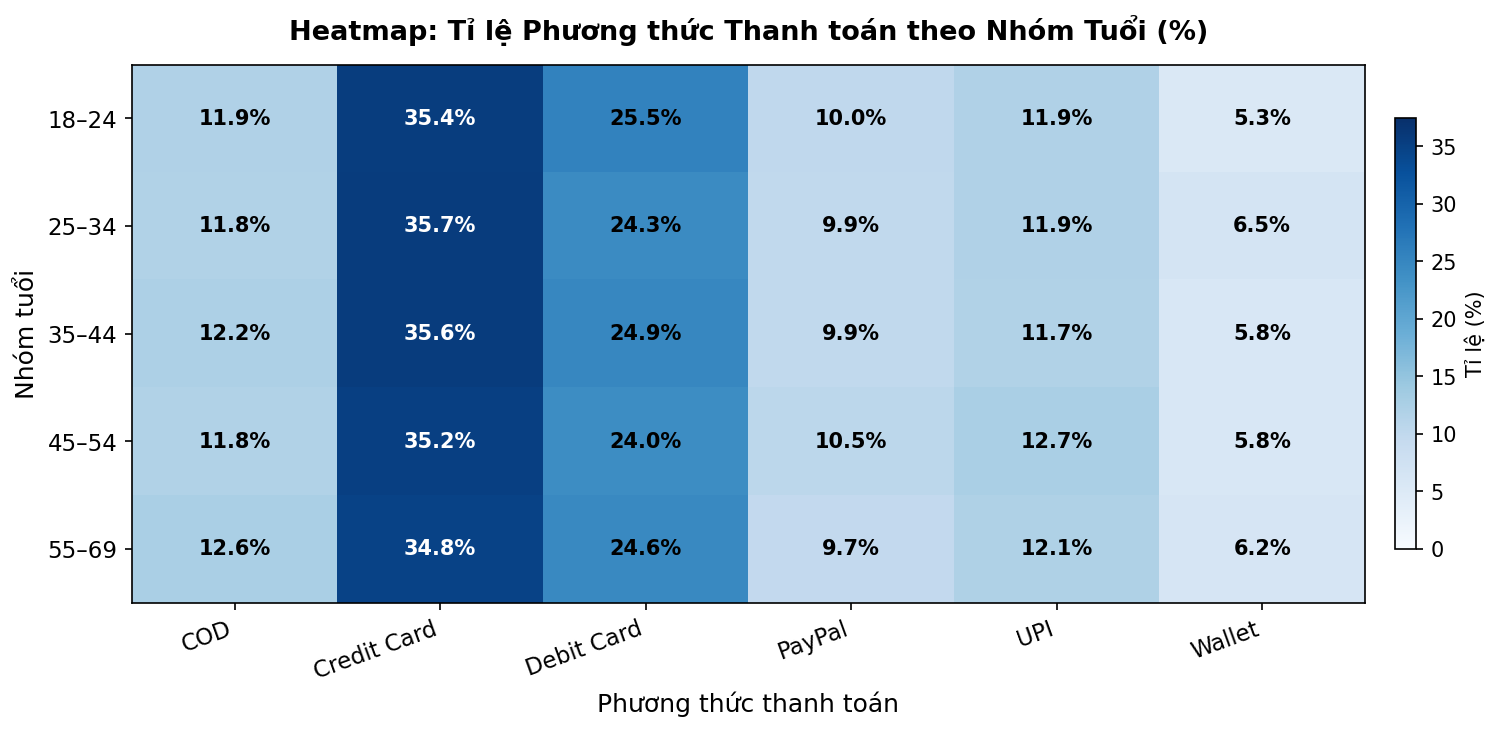
\includegraphics[width=0.9\textwidth]{images/customer_analysis/cust_payment_heatmap.png}
    \caption{Heatmap tỉ lệ phương thức thanh toán theo nhóm tuổi (\%)}
    \label{fig:cust_payment_heatmap}
\end{figure}

\textbf{b. Phương thức thanh toán nào được ưa chuộng nhất? --- Có sự khác biệt theo nhóm tuổi không?}
\\
Biểu đồ \ref{fig:cust_payment_heatmap} trình bày dưới dạng Heatmap với các ô màu xanh (độ đậm tỉ lệ thuận với phần trăm sử dụng) và giá trị \% được ghi trực tiếp trên từng ô. \textbf{Credit Card} là phương thức thống trị ở \textit{tất cả} các nhóm tuổi với tỉ lệ dao động \textbf{35--36\%}, phản ánh sự tin tưởng vào bảo mật thẻ và các ưu đãi hoàn tiền đi kèm. \textbf{Debit Card} xếp thứ hai với khoảng \textbf{24--25\%} và khá đồng đều qua mọi độ tuổi, cho thấy đây là lựa chọn phổ quát không phụ thuộc vào thế hệ. Điểm đáng lưu ý là \textbf{COD (thanh toán khi nhận hàng)} duy trì ổn định ở mức \textbf{$\sim$12\%} và không giảm mạnh ở nhóm cao tuổi như kỳ vọng, điều này cho thấy tâm lý an toàn khi mua sắm trực tuyến vẫn còn phổ biến. \textbf{UPI} và \textbf{PayPal} lần lượt chiếm khoảng \textbf{12\%} và \textbf{10\%} đồng đều qua mọi nhóm --- gợi ý cả hai đã được phổ cập rộng rãi bất kể tuổi tác. \textbf{Wallet} có tỉ lệ thấp nhất ($\sim$6\%) và không có sự chênh lệch rõ rệt theo tuổi, điều này mâu thuẫn với kỳ vọng giới trẻ dùng ví nhiều hơn, có thể do ưu đãi Credit Card hấp dẫn hơn tạo ra hiệu ứng thay thế.

\begin{figure}[H]
    \centering
    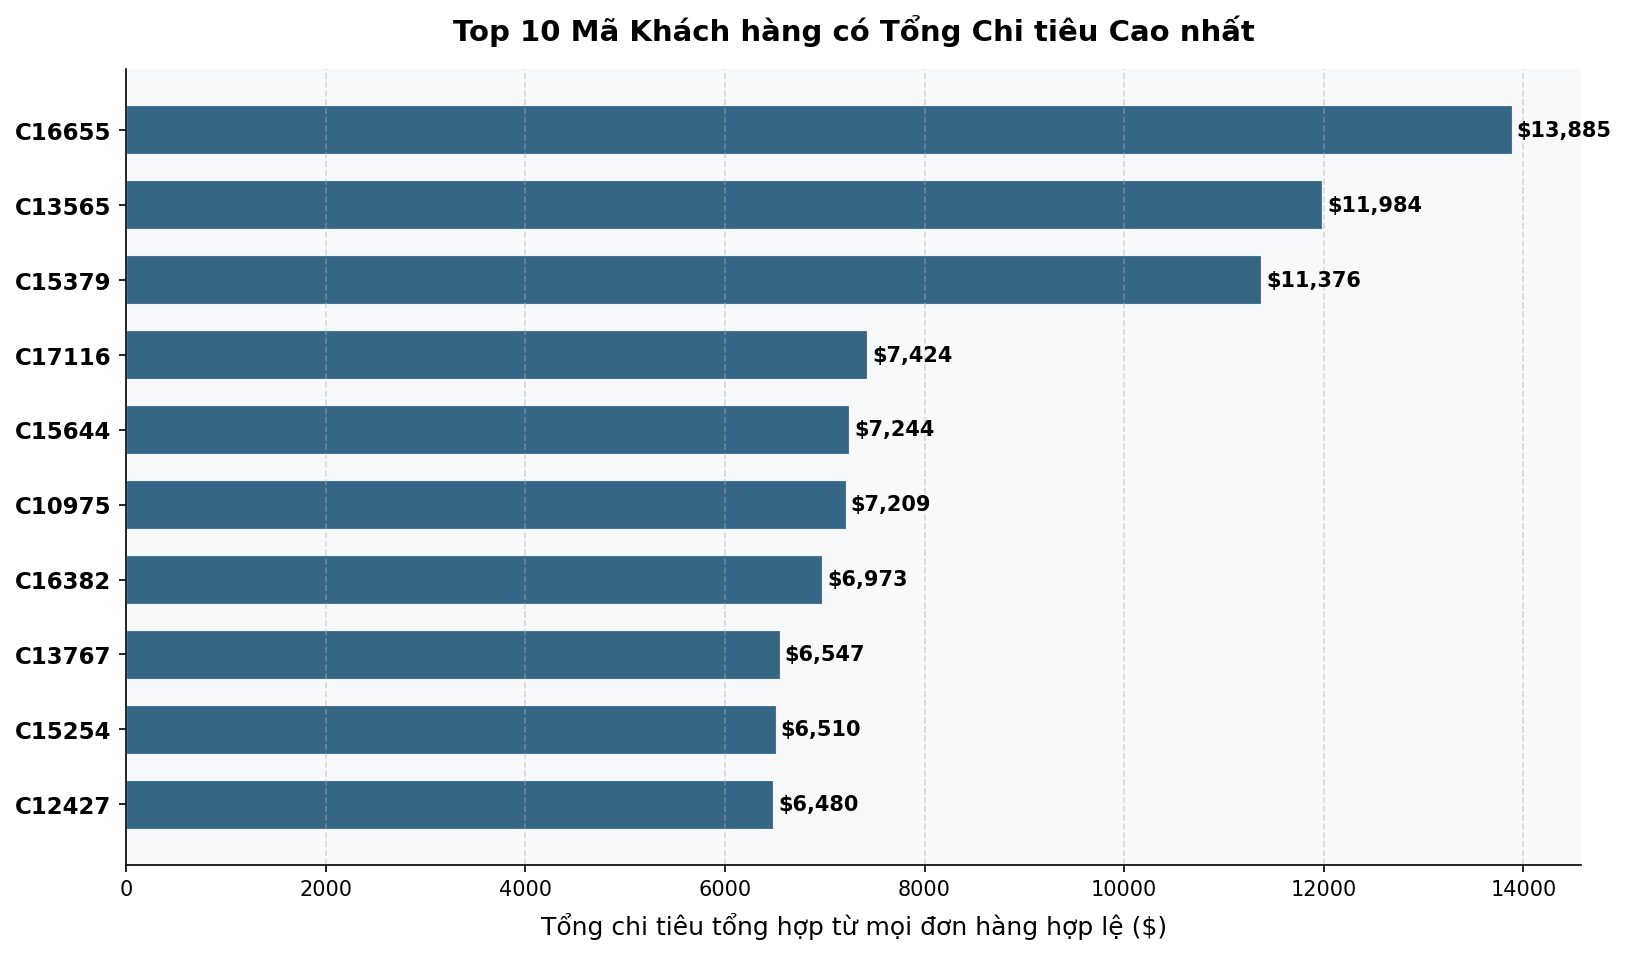
\includegraphics[width=0.9\textwidth]{images/customer_analysis/cust_top10.png}
    \caption{Top 10 khách hàng theo tổng chi tiêu tích lũy (USD)}
    \label{fig:cust_top10}
\end{figure}

\textbf{c. Top khách hàng có giá trị cao nhất (theo tổng chi tiêu) là ai?}
\\
Biểu đồ \ref{fig:cust_top10} sử dụng Horizontal Bar Chart hiển thị, sắp xếp theo tổng chi tiêu thực tế (đã loại trừ đơn hàng hoàn trả) tổng hợp trực tiếp từ mã \texttt{customer\_id}. Khách hàng \textbf{C16655} dẫn đầu cực kỳ ấn tượng với tổng chi tiêu \textbf{\$13,885} --- vượt qua đáng kể so với nhóm bám đuổi, phản ánh mức độ tập trung giá trị cao ở một số ít VIP customer. Việc định danh và phân loại nhóm tinh hoa này sẽ dựa hoàn toàn trên mã \texttt{customer\_id} do biến động về thông tin định dạng cá nhân. Đáng chú ý, toàn bộ 10 định danh xếp đầu bảng này đều đã vượt qua các mốc chi tiêu rất lớn trên sàn, trong đó ngưỡng \textbf{\$6,480} của tài khoản lọt vào top 10 là mốc tham chiếu quan trọng để nền tảng tự động thiết lập chính sách đãi ngộ, trao tặng voucher lớn trong các chương trình khách hàng thân thiết (loyalty programs) sắp tới.

\vspace{0.3cm}
\noindent\textbf{4. Đưa ra quyết định trong tương lai:}
\begin{itemize}
    \item \textbf{Cá nhân hóa marketing cho nhóm VIP:} Xây dựng kịch bản chăm sóc riêng cho thực thể dẫn đầu như khách hàng \textbf{C16655} và nhóm Top 10 để duy trì sự trung thành.
    \item \textbf{Kích cầu nhóm khách hàng trung niên (45--69):} Thiết kế các chiến dịch quảng cáo nhắm mục tiêu vào nhóm tuổi này vì họ có sức mua lớn nhất, đặc biệt là nữ giới trong nhóm 55--69 tuổi.
    \item \textbf{Hợp tác đẩy mạnh thanh toán thẻ:} Liên kết với các ngân hàng để tung ra thêm ưu đãi hoàn tiền (cashback) cho \textbf{Credit Card} vì đây là phương thức chủ đạo được mọi nhóm tuổi tin dùng. Đồng thời, cần cải thiện trải nghiệm \textbf{Wallet} để thu hút thêm đối tượng trẻ tuổi.
\end{itemize}



\subsubsection{Nhóm 4: Phân bổ Khu vực \& Vận chuyển}

\begin{enumerate}
    \setcounter{enumi}{9}
    \item \textbf{Doanh thu phân bổ ra sao theo các khu vực địa lý?} Khu vực nào có hiệu suất tốt nhất?
    \item \textbf{Thời gian giao hàng và chi phí vận chuyển khác nhau thế nào giữa các khu vực?}
    \item \textbf{Có mối tương quan nào giữa chi phí vận chuyển và tỷ lệ hoàn trả không?}
\end{enumerate}

% --- tv4_thevinh.tex ---
% Phân tích Nhóm 4: Phân bổ Khu vực & Vận chuyển

\noindent\textbf{Kết quả phân tích dự kiến:}
\begin{itemize}
    \item Bản đồ nhiệt hoặc biểu đồ cột theo khu vực địa lý.
    \item Thống kê thời gian giao hàng và chi phí vận chuyển.
\end{itemize}


